\section{Vocabulary Supervision: Parameter Updates and Task Performance}
\label{sec:density}

Expanding supervision from one sampled token to a larger vocabulary set changes gradient approximation and task-level learning. We compare sampled-token supervision with the student--teacher top-64 intersection during mathematics-only and joint training. Full-vocabulary supervision supplies a reference for the gradient and single-step comparisons.

\subsection{Broader supervision produces task-dependent gains}

\paragraph{The mathematics advantage develops during training.}
In mathematics-only training, sampled-token supervision leads top-64 by 2.8 accuracy points at update 100; top-64 leads by 2.2 points at update 500 (Figure~\ref{fig:supervision_overview}c). Joint training also ends with a mathematics gain from top-64 supervision, accompanied by a science loss: final differences are $+2.6$ points on mathematics and $-1.2$ on GPQA. Code and instruction-following differences are smaller.

Top-64's joint-training mean advantage narrows from 1.69 points at update 250 to 0.43 at update 500. These trajectories show that the observed benefit depends on the task and the stage of training.

\paragraph{Larger candidate sets redistribute gains across tasks.}
Top-16 and top-64 supervision reach development means of 39.03\% and 39.04\%, and separate-test means of 44.56\% and 44.46\% (Table~\ref{tab:main_outcomes}). On the separate tests, top-64 gains 1.96 mathematics points and loses 2.35 code points relative to top-16.

\begin{figure}[t]
\centering
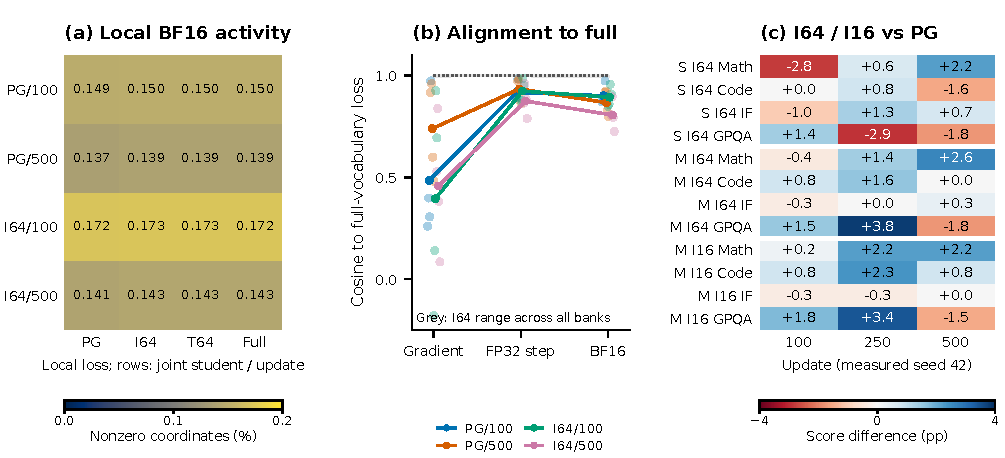
\includegraphics[width=\linewidth]{figures/nine_panel_20260914/section5_supervision.pdf}
\caption{Supervision geometry and capability.
(a) Mean BF16 nonzero fractions by student state and loss.
(b) Alignment with full-vocabulary supervision: PG bank means (lines) and individual banks (points), with the I64 range shaded.
(c) I64-minus-PG task scores (percentage points); positive values favor I64. S/M denote single-teacher/joint training.}
\label{fig:supervision_overview}
\end{figure}


\subsection{Larger candidate sets improve gradient approximation}
\label{sec:coverage_gradient}

Truncating vocabulary support omits probability mass and changes token weights \citep{anshumann2025sparse,huang2026tailaware}. We measure coverage as the student probability retained by the student--teacher candidate intersection, $c_k(h)=\sum_{v\in S\cap T}p_\theta(v\mid h)$, and compare gradients.

\paragraph{Top-64 closely matches the full-vocabulary direction in Qwen.}
The intersection retains over 99.9\% of student probability on average, and its gradient direction is close to that of full-vocabulary supervision (Figure~\ref{fig:supervision_overview}b). Averaging 1, 16, and 64 token samples raises the mean gradient cosine from 0.54 to 0.87 to 0.97; top-64 exceeds 0.999 (Figure~\ref{fig:sampling_history_controls}a). This sampling control identifies finite-sample variation as one source of the directional difference.

\paragraph{Lower-coverage inputs retain appreciable gradient error in SmolLM.}
SmolLM3-3B measurements use the MixSFT initialization and its student after 500 updates of top-64 training with response averaging and three teachers for mathematics, code, and instruction following \citep{gao2026openmopddiagnosingfixingcapability}. Mean top-64 coverage is 97.42\% initially and 98.56\% after training; 8.42\% and 3.65\% of weighted prefixes retain less than 90\% mass (Figure~\ref{fig:smollm_supervision}a,b). Larger candidate sets reduce this low-coverage tail.

We compare gradients on typical prefixes, high-entropy prefixes, and prefixes with top-64 coverage below 99\%. Top-64 has 2.16--24.54\% relative gradient error against full-vocabulary supervision. Top-4 and top-8 produce larger errors in the evaluated batches (Figure~\ref{fig:smollm_supervision}d). Here relative error is the norm of the gradient difference divided by the full-vocabulary gradient norm, capturing both direction and magnitude. Larger candidate sets improve the approximation, with residual error at top-64.

\begin{figure}[t]
\centering
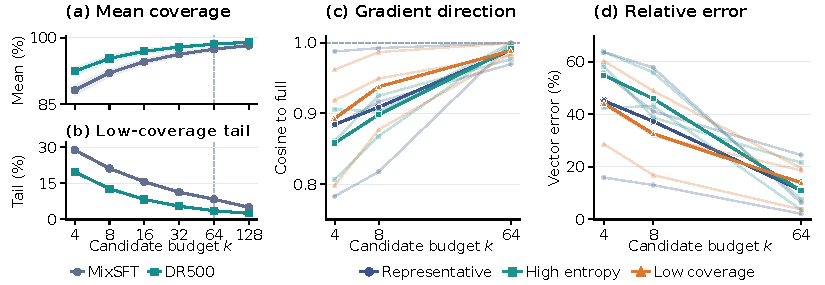
\includegraphics[width=\linewidth]{figures/layout_followup_20260918/smollm_supervision.pdf}
\caption{\textbf{Larger candidate sets improve coverage and gradient approximation in SmolLM.}
(a,b) Mean retained student probability and fraction of inputs below 90\% coverage; bands show response-cluster 95\% intervals. Dashed lines mark top-64.
(c,d) Gradient cosine and relative error against full-vocabulary supervision at the trained student. Groups comprise typical inputs, uncertain next-token predictions, and inputs with lower top-64 coverage; thin lines show batches and bold lines their means. MixSFT/DR500 denote the initialization/trained student.}
\label{fig:smollm_supervision}
\end{figure}

\paragraph{SmolLM capability scores also reveal changes below the aggregate.}
Sampled-token training with SGD raises MATH-500 accuracy from 50.60\% to 53.80\%. On AIME 2025, the initialization, the top-64/domain-token Adam student, and the sampled-token/response-averaged SGD student each solve four of 30 questions with eight samples per question; only one solved question is common to all three.


\subsection{Vocabulary supervision leaves single-step concentration nearly unchanged}

Sampled-token, top-64, teacher-top-64, and full-vocabulary losses produce nearly identical single-step concentration (Figure~\ref{fig:supervision_overview}a). This similarity across vocabulary supports is consistent with concentrated stored-weight changes under dense distillation \citep{yu2026denseupdates}.

The teacher-top-64 reference uses a fixed teacher top-64 set $T$ and full-vocabulary probabilities:
\begin{equation}
\ell_{\mathrm{T64}}=\sum_{v\in T}\left[p_\theta(v)\log\frac{p_\theta(v)}{q_d(v)}-p_\theta(v)+q_d(v)\right].
\label{eq:t64}
\end{equation}
The $-p_\theta(v)$ correction cancels the $+1$ derivative term on this restricted support; $q_d(v)$ is constant with respect to the student and makes each summand zero when $p_\theta(v)=q_d(v)$. Hence $\nabla_\theta\ell_{\mathrm{T64}}=g_T$, using the notation of Section~\ref{sec:setting}. T64 omits terms outside $T$ but has no $1/Z_S$ rescaling, whereas I64 uses $g_I/Z_S$. Neither generally recovers the full-KL gradient. T64 and full KL are single-step references; end-to-end training compares PG, I16, and I64.

Shared optimizer history contributes strongly to the similar concentration. Even a zero current gradient changes about 0.14\% of BF16 parameters in the same comparison, close to the fraction changed by the supervised losses. Resetting Adam's moments changes the amount of BF16 writeback (Figure~\ref{fig:sampling_history_controls}b,c).

\begin{figure}[t]
\centering
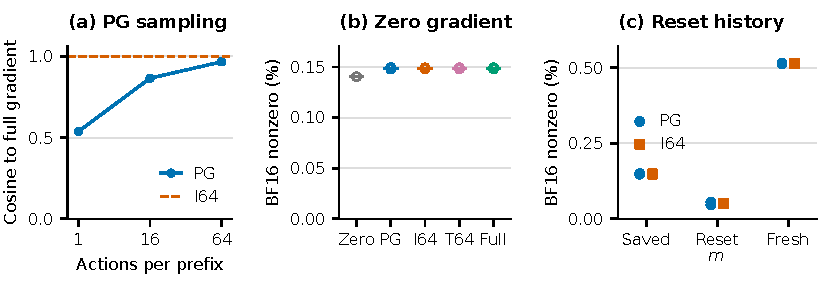
\includegraphics[width=\linewidth]{figures/added_control_figures_20260914/sampling_history_controls.pdf}
\caption{\textbf{More token samples increase PG gradient cosine to full-vocabulary KL; Adam momentum alone changes nearly as many BF16 parameters as PG.}
(a) Gradient cosine to full-vocabulary KL.
(b,c) Nonzero BF16 changes with a zero current gradient or reset Adam moments. Points denote cached batches; bars show means.}
\label{fig:sampling_history_controls}
\end{figure}


Over training, student parameters, responses, and optimizer moments evolve together. Top-64 and sampled-token supervision consequently accumulate different BF16 displacements (Section~\ref{sec:subnetworks}), alongside the task-dependent learning trajectories above.

\FloatBarrier
